
\chapter{"WU"谜题}

\section{形式系统}

本书中心的概念之一是形式系统。我用的这种形式系统是美国逻辑学家艾米尔·波斯特在二十世纪二十年代发明的,通常被称为“波斯特产生式系统”。本章将向读者介绍一个形式系统,并且我希望读者愿意——至少是有一点点愿意——去探索这个形式系统。为唤起读者的好奇心,我设计了一个小小的谜题。

这个谜题就是“你能产生"WU"吗?”。一开始的时候,我提供给你一个符号串(即一串字母)。为了解除你的悬念,可以告诉你那个符号串就是"WJ"。然后,你会得知一些规则,运用这些规则你可以将一个符号串变成另一个。如果某条规则在某处是适用的,并且你也愿意用它,你就可以用。但是,如果同时有几条可以适用的规则,又没有什么指导来说明你该用哪一条,这将留给你去选择。正是这一点使得做形式系统游戏成为一种技巧。重要的、几乎用不着说明的一点是,你决不能做任何背离规则的事情。我们也许可以把这个限制称做“形式化要求”。在本章中,这一点也许根本无需强调。但是我预言——这说起来挺怪的——当你在下面的章节中与形式系统周旋时,你会发现,你将一次又一次地违反形式化要求,除非你以前用过形式系统。

关于我们的形式系统——"WJU"系统——要说的第一件事是它只用了三个字母:"W"、"J"、"U"。就是说"WJU"系统的所有符号串都是由这三个字母组成的。以下是"WJU"系统的一些符号串。
\begin{itemize}
\item "WU"
\item "UJW"
\item "WUUWUU"
\item "UJJUWJUUJWUJJUWJUUJWUJJU"
\end{itemize}
虽然所有这些符号串都是合法的,但它们还不算“归你所有”。事实上,到现在为止归你所有的符号串只有"WJ"。要增加你自己的储备,只能靠使用规则,我们现在就介绍这些规则。下面是第一条规则:

\begin{thm}{规则I}
如果一个归你所有的符号串结尾是"J",则可以在其后面再加上一个"U"。
\end{thm}

这里顺便指出一个事实(假如你到目前还未猜出“符号串”的意思):符号串中的字母是有固定顺序的。比如"WJ"和"JW"是两个不同的符号串。一个符号串不是其字母的顺序无关紧要的“一堆符号”。

以下是第二条规则:
\begin{thm}{规则II}
如果你有$"W"x$,那么$"W"xx$也归你所有。
\end{thm}

我的意思可在下面几个例子里表示出来:
\begin{itemize}
\item 从"WJU",可以得出"WJUJU"。
\item 从"WUW",可以得出"WUWUW"。
\item 从"WU",可以得出"WUU"。
\end{itemize}

就是说,在这条规则中字母“$x$”可以代表任意的符号串。但是,一旦决定了它代表哪一个符号串,就得遵循这个选择(直到你再一次使用这条规则,才可以做一个新的选择)。请注意上面第三个例子。它表明如何在有了"WU"之后,为你的储备增加另一个符号串。但是得先有"WU"!关于字母“$x$”,我想再加上最后一条说明:它不像“"W"”、“"J"”和“"U"”这三个字母一样,是形式系统的一部分。无论如何,如果我们能有某种符号的方式一般性地谈论系统中的符号串,那将是很有用的——而“$x$”正是起了这个作用:代表任意一个符号串。假如在你的符号串“储备”中加入一个含有“$x$”的符号串,那就错了,因为"WJU"系统中的符号串决不会带有“$x$”!

以下是第三条规则:
\begin{thm}{规则III}
如果"JJJ"出现在你的储备中的一个符号串里,那么你可以用"U"代替这个"JJJ"而得到一个新的符号串。
\end{thm}
例子:
\begin{itemize}
\item 从"UWJJJWU",可以得到"UWUWU"。
\item 从"WJJJJ",可以得到"WJU"\lnote{(同样可以得到"WUJ")}。
\item 从"JJWJJ",用这条规则什么也得不到\lnote{(三个"J"必须是连续的)}。
\item 从"WJJJ",可以得到"WU"。
\end{itemize}
在任何情况下,这条规则都不能倒过来使用,像下面的例子里这样:
\begin{itemize}
\item 从"WU",得到"WJJJ"。\hfill $\Longleftarrow$ 这是错误的。
\end{itemize}
规则是单向的。

下面是最后一条规则:
\begin{thm}{规则IV}
如果"UU"出现在你的一个符号串中,你可以去掉它。
\end{thm}

\begin{itemize}
\item 从"UUU",可以得"U"。
\item 从"WUUUJJJ",可以得到"WUJJJ"。
\end{itemize}
规则就是这些。现在可以试试找出"WU"了。假如得不出来不要担心。只是试一下——主要是体会一下"WU"谜题的味道。愿读者从中获得享受。

\section{定理、公理、规则}

"WU"谜题的答案后面会给出来。至于现在,重要的不是找出答案,而是寻找它。读者也许已经做了一些产生"WU"的尝试。在做这些尝试的过程中,读者建立了自己的符号串储备。我们把这种可以从规则中产生的符号串叫做定理。当然,“定理”这个词在数学中也使用,但与这里的意思很不一样。那里的意思是普通语言中的某个陈述,已通过严格的论证被证明是真的(这时我们称之为“真理”),例如,关于“运动无有”的\emph{芝诺定理},或者关于素数有无穷多个的\emph{欧几里德定理}。但是,在形式系统中,不必把定理看做是陈述——它们仅仅是一些由符号组成的串。它们也不是证明出来的,而是产生出来的,就像是按照一定的印刷规则通过机器产生出来的一样。为了强调“定理”这个词在意义上的重要区别,在本书中我将采用以下约定:当“定理”这个词用黑体字写出来时,它的意思是我们通常所说的意思——一个\emph{定理}是日常语言中的一个陈述,这个陈述已被某人用某种逻辑的论证证明是真理。如果不用黑体则“定理”这个词有它的技术上的意义:可以在某个形式系统中产生出来的符号串。在这样的情况下,"WU"谜题是问"WU"是不是"WJU"系统中的一个定理。

开始的时候我无偿地提供了一个定理,即"WJ"。这个“无偿提供的”定理叫做“公理”——同样的,这是技术上的意义,它与通常的意义很不一样。一个形式系统中可以有零个、一个、几个、甚至无穷多个公理。本书中将会出现所有这些不同类型的形式系统。

每一个形式系统中都有符号变换规则,如"WJU"系统中的四条规则。这些规则既可以叫做生成规则,也可以叫做推理规则。这两种叫法我都用。

我在这里要介绍的最后一个术语是推导。以下是一个定理"WUJJU"的推导:

\begin{enumerate}
\setaitem{.3\linewidth}
\aitem "WJ"      \> 公理
\aitem "WJJ"     \> 使用规则II,从(1)中得出
\aitem "WJJJJ"   \> 使用规则II,从(2)中得出
\aitem "WJJJJU"  \> 使用规则I,从(3)中得出
\aitem "WUJU"    \> 使用规则III,从(4)中得出
\aitem "WUJUUJU" \> 使用规则II,从(5)中得出
\aitem "WUJJU"   \> 使用规则IV,从(6)中得出
\end{enumerate}

一个定理的推导说明如何按照这个形式系统中的规则逐行生成该定理的一个明显的论证。“推导”这一概念是向“证明”概念看齐的,但比后者要朴素一些。如果说证明出了"WUJJU",听起来就很奇怪,但是如果说推导出了"WUJJU",就不那么奇怪了。

\section{系统内外}

多数人解"WU"谜题的办法是:先相当盲目地推出一些定理,看一看得到的会是什么。很快地,他们就开始注意到他们产生出的定理的一些性质,人的智能就在此处起作用了。例如,也许你在试开头的几次时,并不清楚所有的定理都是以"W"开头的。推了一阵以后,这个模式浮现在你脑海中。你不仅可以看出这个模式,而且通过检查那些规则,还可以理解这个模式。那些规则有一个性质,即:新产生的定理都继承了原先的那条定理的第一个字母。归根到底,所有的定理的第一个字母都可以追溯到唯一的公理"WJ"的第一个字母——这是一个证明,指出"WJU"系统中所有的定理都必须以"W"开头。

这里发生的情况是有着重要意义的。它展示了人与机器之间的一种区别。非常可能——事实上很容易——给一部计算机编一个程序,使它可以生成"WJU"系统的一条又一条定理,并且我们可以在这个程序中加进一条命令,使之在生成"U"之后才停止。现在你知道了:运行这个程序的计算机会永不停止,而这并不使你感到惊异。但是,假如你要让你的一位朋友试图生成"U",将会怎么样呢?要是他做了一会儿就罢手不干了,跑来向你抱怨他无法摆脱第一个字母"W",而想生成"U"完全是徒劳的,你同样不会吃惊。即使是一个不很聪明的人,也会禁不住地观察他自己在做什么,这些观察给予他关于所做的这项工作的洞察力。而计算机程序——正如我们所描述过的——则缺乏这种洞察力。

现在让我更清楚地谈谈我说“这展示出了人与机器之间的区别”是什么意思。我的意思是:有可能给机器编一个以上述方式来做机械工作的程序,机器永远不会发现(即便这是非常明显的)它自己在做什么。但是人的意识有一个固有的特点,他总是能看出关于他正在做的事情的某些事实。关于这一点,你是早已知道的。假如你在加法机上按一下“$1$”,然后再加$1$,再加$1$,再加$1$,再加$1$……如此一直加上几个小时又几个小时,虽然任何人都会很快地懂得自己在重复一个动作,而那台机器却永远不懂得在你按$1$之前,自己去加。或者,另举一个愚蠢点儿的例子:无论用了多久,无论多好的一部汽车,也永远不会有躲避道路上的其它汽车或障碍物的能力,永远不会知道它的主人常走的路线。

因此,区别在于:机器有可能在做某件事情时不去观察,而人不可能不去观察。请注意,我不是说所有的机器都不具有复杂的观察能力,只是有些机器不具有。我也不是说所有的人都总是进行复杂的观察,事实上,人常常是不注意观察的。但是机器可以被制造成是完全不去观察的,而人则不能。并且事实上,到目前为止,多数机器是非常接近于不去观察的。也许因为这个原因,对于大多数人来说,具有“不去观察”这一特点,似乎是机器的特征。例如,如果有人说某项工作是“机械的”,这指的不是人没有做这项工作的能力,而是隐含着这样的意思:只有机器可以永不抱怨或者不知疲倦地反复做这项工作。

\section{跳出系统}

能够跳出正在进行的工作并且看一下已经做了些什么,这是智能固有的特点。它总是寻找并且常常能找到模式。我说的是智能可以跳出它所做的工作,这不意味着它总是这样做。然而,常常是略微推动它一下就足够了。就好比一个正在读书而感觉困倦的人,他不是连续地把这本书看完,而可能把书搁在一边儿,把灯关掉。他“出了系统”,而这对我们来说似乎是再自然不过的了。或者,假设一个人,A,正在看电视,B进了屋子,并且明显地表示出对于当时的状况不喜欢。A可能认为他理解了问题的所在,并且试图通过从当前系统(那时的电视节目)退出来改变一下现状,于是他轻轻按了一下频道钮,找一个好一点儿的节目。不过B可能对于什么是“退出系统”有更极端的概念——也就是,把电视机关掉!当然也有这种情况:只有极少数的人有那种眼光,看出一个支配着许多人生活的系统,而以前却从没人认为这是一个系统。然后这些人常常就投入毕生的精力去使其他人相信那个系统确实存在,而且应该从中退出!

若想教给计算机跳出系统这件事,能教会它到什么程度呢?我举一个使一些人吃惊的实例:不久以前,在加拿大举行的一次计算机国际象棋邀请赛上,一个程序——所有竞争者中最弱的一个——有一个非同一般的特性:它可以远在棋下完之前早早退出。它的棋下得不太好,但它至少有预先估计到没有希望的棋局的能力,然后就此停下,而不是等着另一个程序走完将死它的乏味的过程。虽然每次下棋它都输,但是它做得很有风度。它给很多当地的下棋能手留下了深刻的印象。假如把“系统”定义成“在下棋的游戏中走棋的系统”,那么,很清楚,这个程序有一个很复杂的事先编好的有能力从系统中退出的程序。另一方面,如果把“系统”定义成“这部计算机按照程序所做的一切”,那么无疑地,这部计算机没有什么从那个系统中退出的能力。

在研究形式系统时,很重要的一点是要区分在系统之内的工作,和做出关于系统的判断或说明。我假定读者像大多数人一样,开始时,想通过在系统内部工作解决"WU"谜题;逐渐地,你开始着急了,这种焦急心情增长到一定程度时就不再作任何考虑地退出了这个系统,然后盘算一下产生了一些什么,想想为什么没有取得成功——即产生出"WU"。也许你发现了没能产生出"WU"的原因所在,这是对于系统进行思索。也许你在中途什么时候产生了"WJU",这是在系统之内进行工作。我不想把事情弄得好像两种方式完全不相容,我敢肯定任何一个人都有某种程度的在系统之内进行工作,同时思考他正在做什么的能力。实际上,在人类事务中,通常是几乎不可能将“在系统之内”和“在系统之外”清楚地区别开的,生活是由许多连结并交织又常常是不协调的“系统”组成的,用“系统内”、“系统外”这类词汇来思考似乎是过于简单化了。但是,非常清楚地形成一些简单的概念,以便人们可以在思考更复杂的概念时把它们作为模型,这常常是重要的。这便是我为什么要向读者展示形式系统的原因。现在是回头讨论"WJU"系统的时候了。

\section{"W"方式、"J"方式、"U"方式}

"WU"谜题的陈述方式鼓励人们在"WJU"系统内部进行探索——做一些定理推导。但这个问题的陈述方式并不暗示在系统之内必然会产生结果。因此它使得人们往返于两种方式之间。一个把两种方式区分开的方法可以是:准备两张纸,在一张纸上,你“像机器那样”地工作,这样在纸上写满了的都是"W"、"J"、"U"这三个字母。在另一张纸上,你“像有思维能力的人那样”地工作,你可以做你的智能要你做的任何事情——可以使用汉语、记下要点、进行逆推、使用缩写(比如使用字母“$x$”)、把几个步骤缩成一步、把规则加以修改看看可以得出什么东西,以及做你所能想象到的任何其它事情。要注意$3$和$2$这两个数起着很重要的作用,因为,三个"J"是可以扔掉的,两个"U"也可以去掉。另外根据规则II,可以把长度延长一倍(除了那个"W")。所以第二张纸上也可以有一些计算。我们会时常重新提到处理形式系统的这两种方式,我们分别称之为机方式("J"方式)和惟方式("W"方式)。为了完满,使"WJU"系统的每一个字母都与一种方式相关联,我再提出最后一种方式——无方式("U"方式),它是禅宗的处世态度。关于这点在后面几章中会更多地讲到。

\section{判定过程}

对于这个谜题的观察表明,它涉及到两种具有不同趋向的规则——加长的规则和缩短的规则。其中两条规则(规则I和II)允许你加长符号串(当然只能是非常刻板地按预先规定的方式来加长),另外两条规则允许多少缩短一点符号串(同样是以非常刻板的方式)。看起来应该是有无限多种不同的顺序来应用这些不同种类的规则,这就使得用这种或那种方式来产生"WU"有了希望。可能是使符号串加长成一个庞然大物,然后再一段一段地抽掉,直到只剩下两个符号为止;或者更糟糕,使符号串连续地加长、缩短、再加长、再缩短,如此下去,而结果如何却没有保证。事实上,我们已经看出"U"是不可能产生的,即使是加长或缩短到世界末日也无济于事。

然而,"U"和"WU"似乎很不相同。通过"U"的非常表面的特征,我们可以辨别出不可能产生它:它不是以"W"开头的(而所有的定理都必须是)。用这样一个简单的方法去发现非定理是很方便的。然而,能说这个测试可以发现出所有的非定理吗?可能会有许多以"W"开头但无法产生的符号串。也许"WU"就是其中之一。这也就是说“字头测试”的用途是有限的,它只能发现一部分非定理,而漏掉其它的。但是仍然有可能有一些更精细的测试,这些测试完全能区分哪些符号串通过规则可以产生,哪些不能产生。这里我们得面对一个问题:“我们的测试是什么意思?”目前这个问题的意义或者重要性也许不明显。下面我举一个关于“测试”的例子,某种意义上似乎有点违反这个词的精神:

设想在这个世界上有一个怪物,它有足够的时间,并且喜欢把时间用来以有秩序的方法去产生"WJU"系统的定理。例如,下面就是这个怪物可能采取的一种方式:

\begin{enumerate}[step]
\item 对于公理"WJ"应用每一条可以应用的规则。这产生出两个新的定理:"WJU"、"WJJ"。
\item 对于从步骤1中产生的定理应用所有可以应用的规则。这产生出三个新的定理:"WJJU"、"WJUJU"和"WJJJJ"。
\item 对于步骤2中产生的定理应用所有可以应用的规则。这产生出五个新的定理:"WJJJJU"、"WJJUJJU"、"WJUJUJUJU"、"WJJJJJJJJ"和"WUJ"。
\item[{\makebox[\labelwidth]{$\vdots$}}]
\end{enumerate}
这种方法早晚会产生出所有的定理,因为每条规则都在任意能设想出的次序下应用过。(参看\fig{11})我们以上提到的所有那些加长——缩短的交替用法最终都用上了。然而对于一个给定的符号串,就不知道要经过多少步它才能出现在这张表里,因为定理是按照它们的推导长度来列出的。这不是一个很有用的次序,假如你对一个特殊的符号串(像"WU")感兴趣的话,你甚至不知道是否有个推导能得出它,更不知道那个推导会有多长了。

\begin{figure}
%\includegraphics{img_011.png}
\begin{tikzpicture}[thick, node distance=10mm and 2mm,
  inner sep=0mm,outer ysep=.3333em,
  sibling distance=5mm, level distance=7mm,
  quan/.style={decorate, decoration={markings,
    mark connection node=quan,
    mark=at position .5 with
      {\node[circle, draw, inner sep=.8pt, outer sep=0pt]
            (quan) {#1};}}}]
\node (A) {"WJUJUJUJU"}
  child;
\node (B) [right = of A] {"WJJUJJU"}
  child;
\node (C) [right = of B] {"WJJJJU"}
  child foreach \x in {1,2,3};
\node (D) [right = of C] {"WJJJJJJJJ"}
  child[sibling distance=3mm] foreach \x in {1,2,...,8};
\node (E) [right = of D] {"WUJ"}
  child
  child;
\node (F) [right = of E] {"WJU"}
  child;
\node (G) [above = of A] {"WJUJU"}
  edge[quan=2] (A);
\node (H) [above = of B] {"WJJU"}
  edge[quan=2] (B);
\node (I) at ({$(C)!.5!(F)$} |- H) {"WJJJJ"}
  edge[quan=1] (C)
  edge[quan=2] (D)
  edge[quan=3] (E)
  edge[quan=3] (F);
\node (J) [above = of G] {"WJU"}
  edge[quan=2] (G);
\node (K) at ({$(H)!.5!(I)$} |- J) {"WJJ"}
  edge[quan=1] (H)
  edge[quan=2] (I);
\node (L) [above = of $(J)!.5!(K)$] {"WJ"}
  edge[quan=1] (J)
  edge[quan=2] (K);
\path[font=\bfseries]
  node[name=M, left = 2mm of A] {3.}
  (M |- G) node {2.}
  (M |- K) node {1.}
  (M |- L) node {0.};
\node[name=O, below left = 15mm of current bounding box.north east] {"WU"};
\tikzset{shift={(O)}}
\node foreach \x in {30,90,...,330} at (\x:8mm) {?};
\end{tikzpicture}
\caption["WJU"系统中所有定理的“树”。]
  {一个系统地构造出来的"WJU"系统中所有定理的“树”。向下到第$N$步,它包含了恰恰需要$N$个步骤推导的那些定理。圆圈中的数字字表示使用了哪条规则。"WU"是不是在这棵树上的什么地方?}
\end{figure}
现在我们给出这个所谓的“定理性测试”:

等待产生出所要求的符号串,当它出现了的时候,你知道它是一个定理——假如它永远不出现,它就不是一个定理。

这看起来是荒唐的,因为它预先假设了我们为了得到一个答案,并不在乎等待哪怕是无限长的时间。这就是该把什么算作“测试”这个问题的关键。最首要的问题是保证我们将在一个有限长的时间内得到答案。如果有一个检验定理的测试,一个总是在有限长的时间内终结的测试,那么,这个测试就叫做给定形式系统的判定过程。

当你有了一个判定过程,那么你就有了对系统中所有定理的性质的非常具体的刻划。从表面上看,似乎形式系统中的规则与公理同判定过程一样完全地刻划了这个系统中的定理。问题在于“刻划”这个词。当然那些推理规则与"WJU"系统中的公理是隐含地刻划了那些是定理的符号串。不仅如此,它们还以更隐蔽的方式刻划了那些非定理的符号串。但是,在许多情况下,隐含地刻划还不够。如果有人声称有了一个对所有定理的刻划,但是若要推断某一个特别的符号串不是一个定理则需要无限长的时间,你大概会倾向于说,这个刻划中缺少点什么——它不够具体。这就是为什么发现判定过程的存在是非常重要的一步。所谓发现,从效果上看就是:你可以为检验一个符号串是不是一个定理进行一种测试,即便这个测试很复杂,它也是保证有结果的。原则上,这个测试与检查符号串的第一个字母是不是"W"同样地容易,同样地机械,同样地有限,同样是十分确定的。一个判定过程是测试一个符号串是否是定理的“试纸”。

顺便说一下,对形式系统的一个要求是,其中的公理必须具有判定过程——必须存在有关于一个符号串是不是一条公理的试纸。这就保证了至少在一开始进行的时候没有问题。这就是一组公理与一组定理之间的区别:前者总是有一个判定过程的,后者则可以没有。

我敢保证你会同意,当你第一次看见"WJU"系统时,你必须得面对这个问题。单独一个公理是已知的,推理规则是简单的,因此定理被隐含地刻划了——然而它仍然不很清楚,你不知道这个刻划的结果是什么。尤其是,"WU"究竟是不是一个定理,这一点仍然不清楚。

\begin{figure}
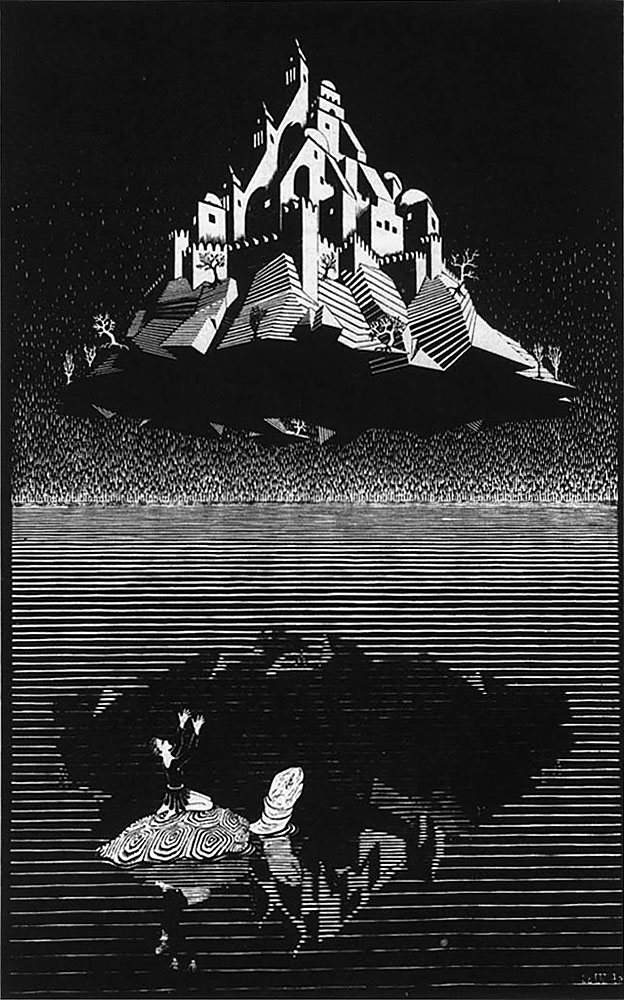
\includegraphics{img_012.jpg}
\caption[空中城堡,艾舍尔作。]
  {空中城堡,艾舍尔作(木刻,1928)。}
\end{figure}

